\interlude[2]<Trials \textasciitilde\ Attacks found>{ChronoTrigger}
\section{State Disruption}

% \begin{frame}[light]{}
%   \vspace{1cm}
%   \large
%   \vollkorn

%   \begin{columns}[fullwidth]
%     \begin{column}{.1\linewidth}
%     \end{column}

%     \begin{column}{.35\linewidth}
%         % …that denial of service can happen on the level of cryptography protocols!

%         % \vfil
%         % …that the wall clock is not to be trusted.

%         % \vfil
%         % …how to accept replay attacks and face them without fear!

%         In the following slides you will learn …
%         \par\vspace{1.5em}
%         how to perform a protocol-level DoS attack against WireGuard,
%         why wall clocks are not to be trusted and how to face replay
%         attacks without fear.
%     \end{column}
%     \begin{column}{.20\linewidth}
%       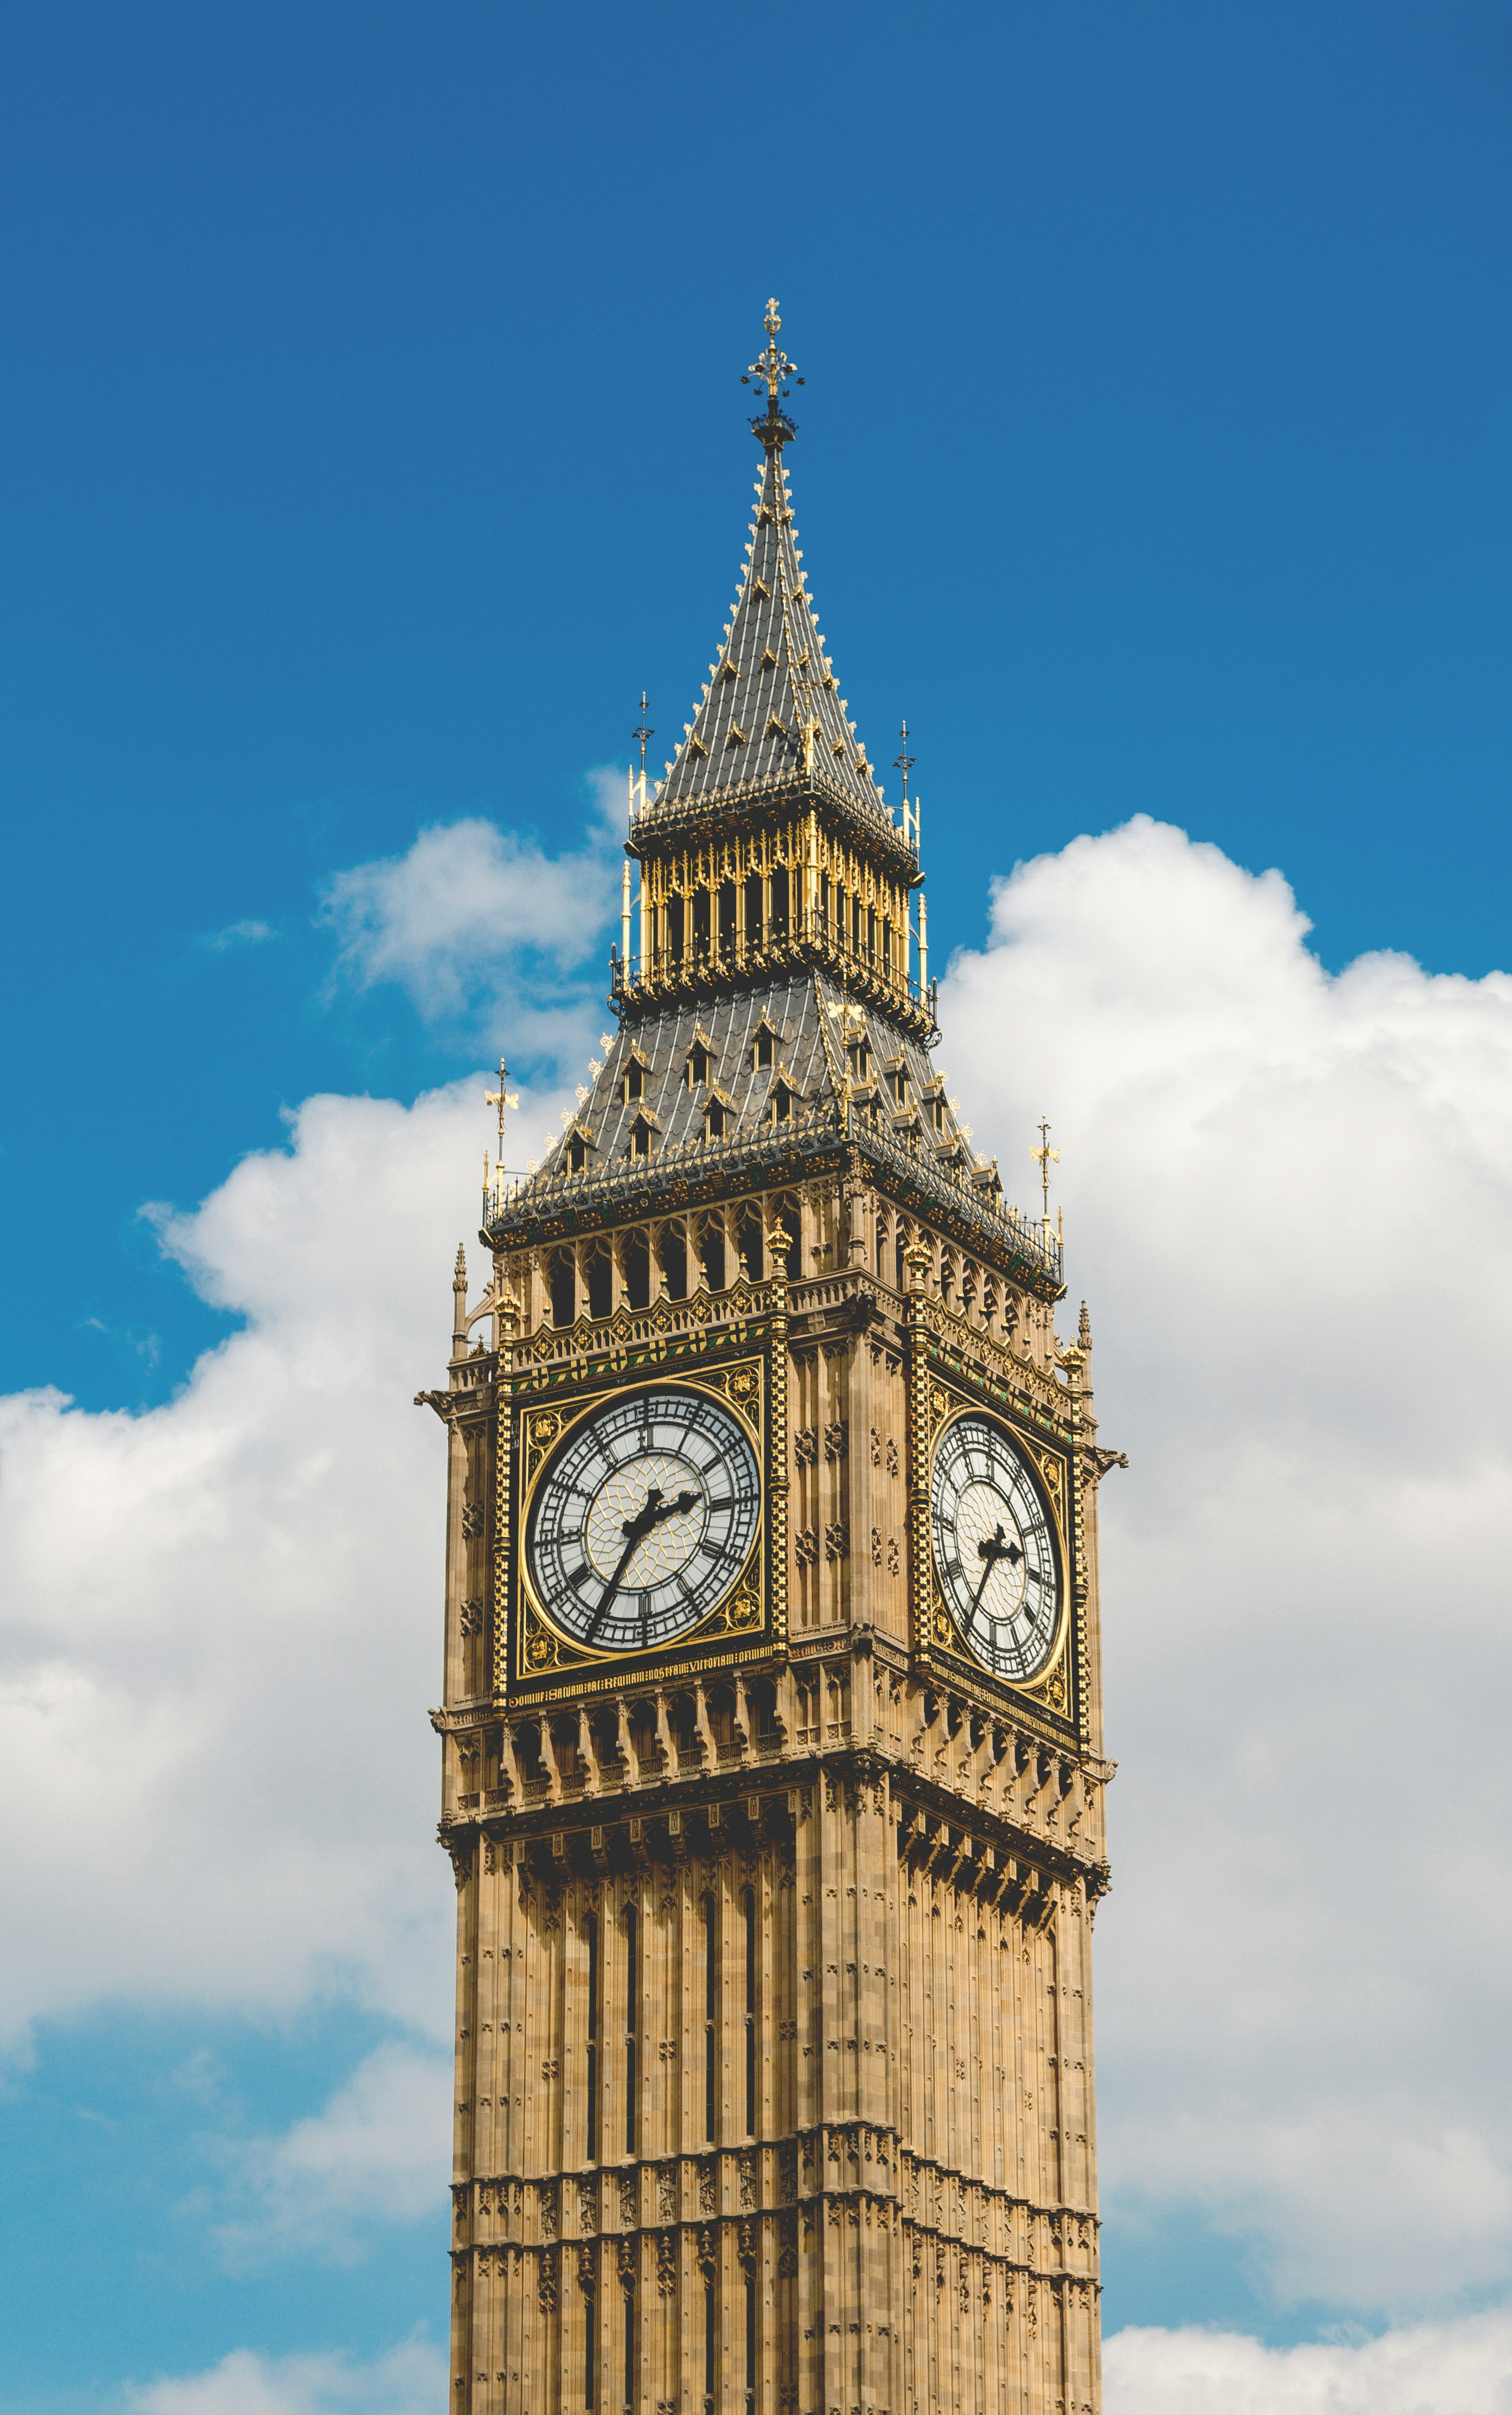
\includegraphics[width=\linewidth]{graphics/big-ben.jpg}
%       \vspace{0.4cm}
%     \end{column}
%     \begin{column}{.20\linewidth}
%       \vspace{1.6cm}
%       \includegraphics[width=\linewidth]{graphics/sad-bunny-looking-left.jpg}
%     \end{column}

%     \begin{column}{.1\linewidth}
%     \end{column}
%   \end{columns}
% \end{frame}


\begin{frame}[T]{Retransmission Protection in WireGuard}
\begin{columns}[fullwidth,T]
  \begin{column}{.5\linewidth}
    \rlap{\includegraphics[height=\extendedframetextheight,page=3,clip=true,trim=0 47 0 50]{rosenpass-wireguard-attack-types}}
  \end{column}
  \begin{column}{.46\linewidth}
  \small
    \begin{itemize}
      \item replay attacks thwarted by counter
      \item counter is based on real-time clock
      \item responder is semi-stateful (one retransmission at program start may be accepted, but this does not affect protocol security)
      \item[$\Rightarrow$]
         WG requires \emph{either} reliable real-time clock \emph{or} stateful initiator
      \item[$\Rightarrow$]
        adversary can attempt replay, but this cannot interrupt a valid handshake by the initiator
      \item[!] Assumption of reliable system time is invalid in practice!
    \end{itemize}
  \end{column}
\end{columns}
\end{frame}




\begin{frame}[T]{ChronoTrigger Attack}
\begin{columns}[fullwidth,T]
  \begin{column}{.5\linewidth}
    \rlap{\includegraphics[height=\extendedframetextheight,page=5,clip=true,trim=0 47 0 50]{rosenpass-wireguard-attack-types}}
  \end{column}
  \begin{column}{.46\linewidth}
      \stretchcolumn{
    \small\leavevmode
    \only<+|handout:+>{

      \begin{enumblock}{Preparation phase:}
      \begin{enumerate}
        \item \textbf{Attacker} sets \emph{initiator system time} to a future value
        \item \textbf{Attacker} records \emph{InitHello} as \emph{KillToken} while both peers are performing a valid handshake
      \end{enumerate}
      \unskip
      \end{enumblock}
      \unskip
      \vfill
\centerline{ \small … both peers are being reset … }
      \begin{enumblock}{Delayed execution phase:}
      \begin{enumerate}
        \item \textbf{Attacker} sends \emph{KillToken} to responder, setting their timestamp to a future value
        \item[$\Rightarrow$] Initiation now fails again due to timestamp mismatch
      \end{enumerate}
      \unskip
      \end{enumblock}
      \unskip
	}

    \only<+|handout:+>{%
      \begin{block}{Gaining access to system time:}
      \begin{itemize}
        \item Network Time Protocol is insecure,\\
        mitigations are of limited use
        \item[$\Rightarrow$] break NTP \emph{once}; kill token lasts forever
      \end{itemize}
      \unskip
      \end{block}
    }

    \only<+|handout:+>{%
      \leavevmode\begin{block}{Attacker gains}
      \begin{itemize}
        \item extremely cheap protocol-level DoS
      \end{itemize}
      \unskip
      \end{block}

      \begin{block}{Preparation phase, attacker needs:}
      \begin{itemize}
        \item eavesdropping of initiator packets
        \item access to system time
      \end{itemize}
      \unskip
      \end{block}

      \begin{block}{Delayed execution, attacker needs:}
      \begin{itemize}
        \item no access beyond message transmission to responder
      \end{itemize}
      \unskip
      \end{block}
  }
}
  \end{column}
\end{columns}
\end{frame}

\begin{frame}{What are State Disruption Attacks?}
      \begin{columns}
        \begin{column}{.3\linewidth}
		\stretchcolumn{\vfill
          \leavevmode\reflectbox{
\includegraphics[width=\linewidth,height=.454\textheight,right,clip,trim={0cm 16cm 0cm 40cm}]{bunny-2.jpg}}%
          }
        \end{column}
        \hfill
        \begin{column}{.38\linewidth}
     \leavevmode\rlap{\raisebox{-.5\height}[.5\height][.5\height]{\includegraphics[width=\linewidth,height=\extendedframetextheight,trim={7cm 38cm 5cm 10cm},clip]{wires.jpg}}}%
	\setlength{\fboxsep}{2ex}%
	\makebox[\linewidth]{\colorbox{white}{\makebox[1.1\linewidth]{%
         \Large Protocol-level DoS
     }}}
        \end{column}
        \hfill
        \begin{column}{.3\linewidth}
          \stretchcolumn{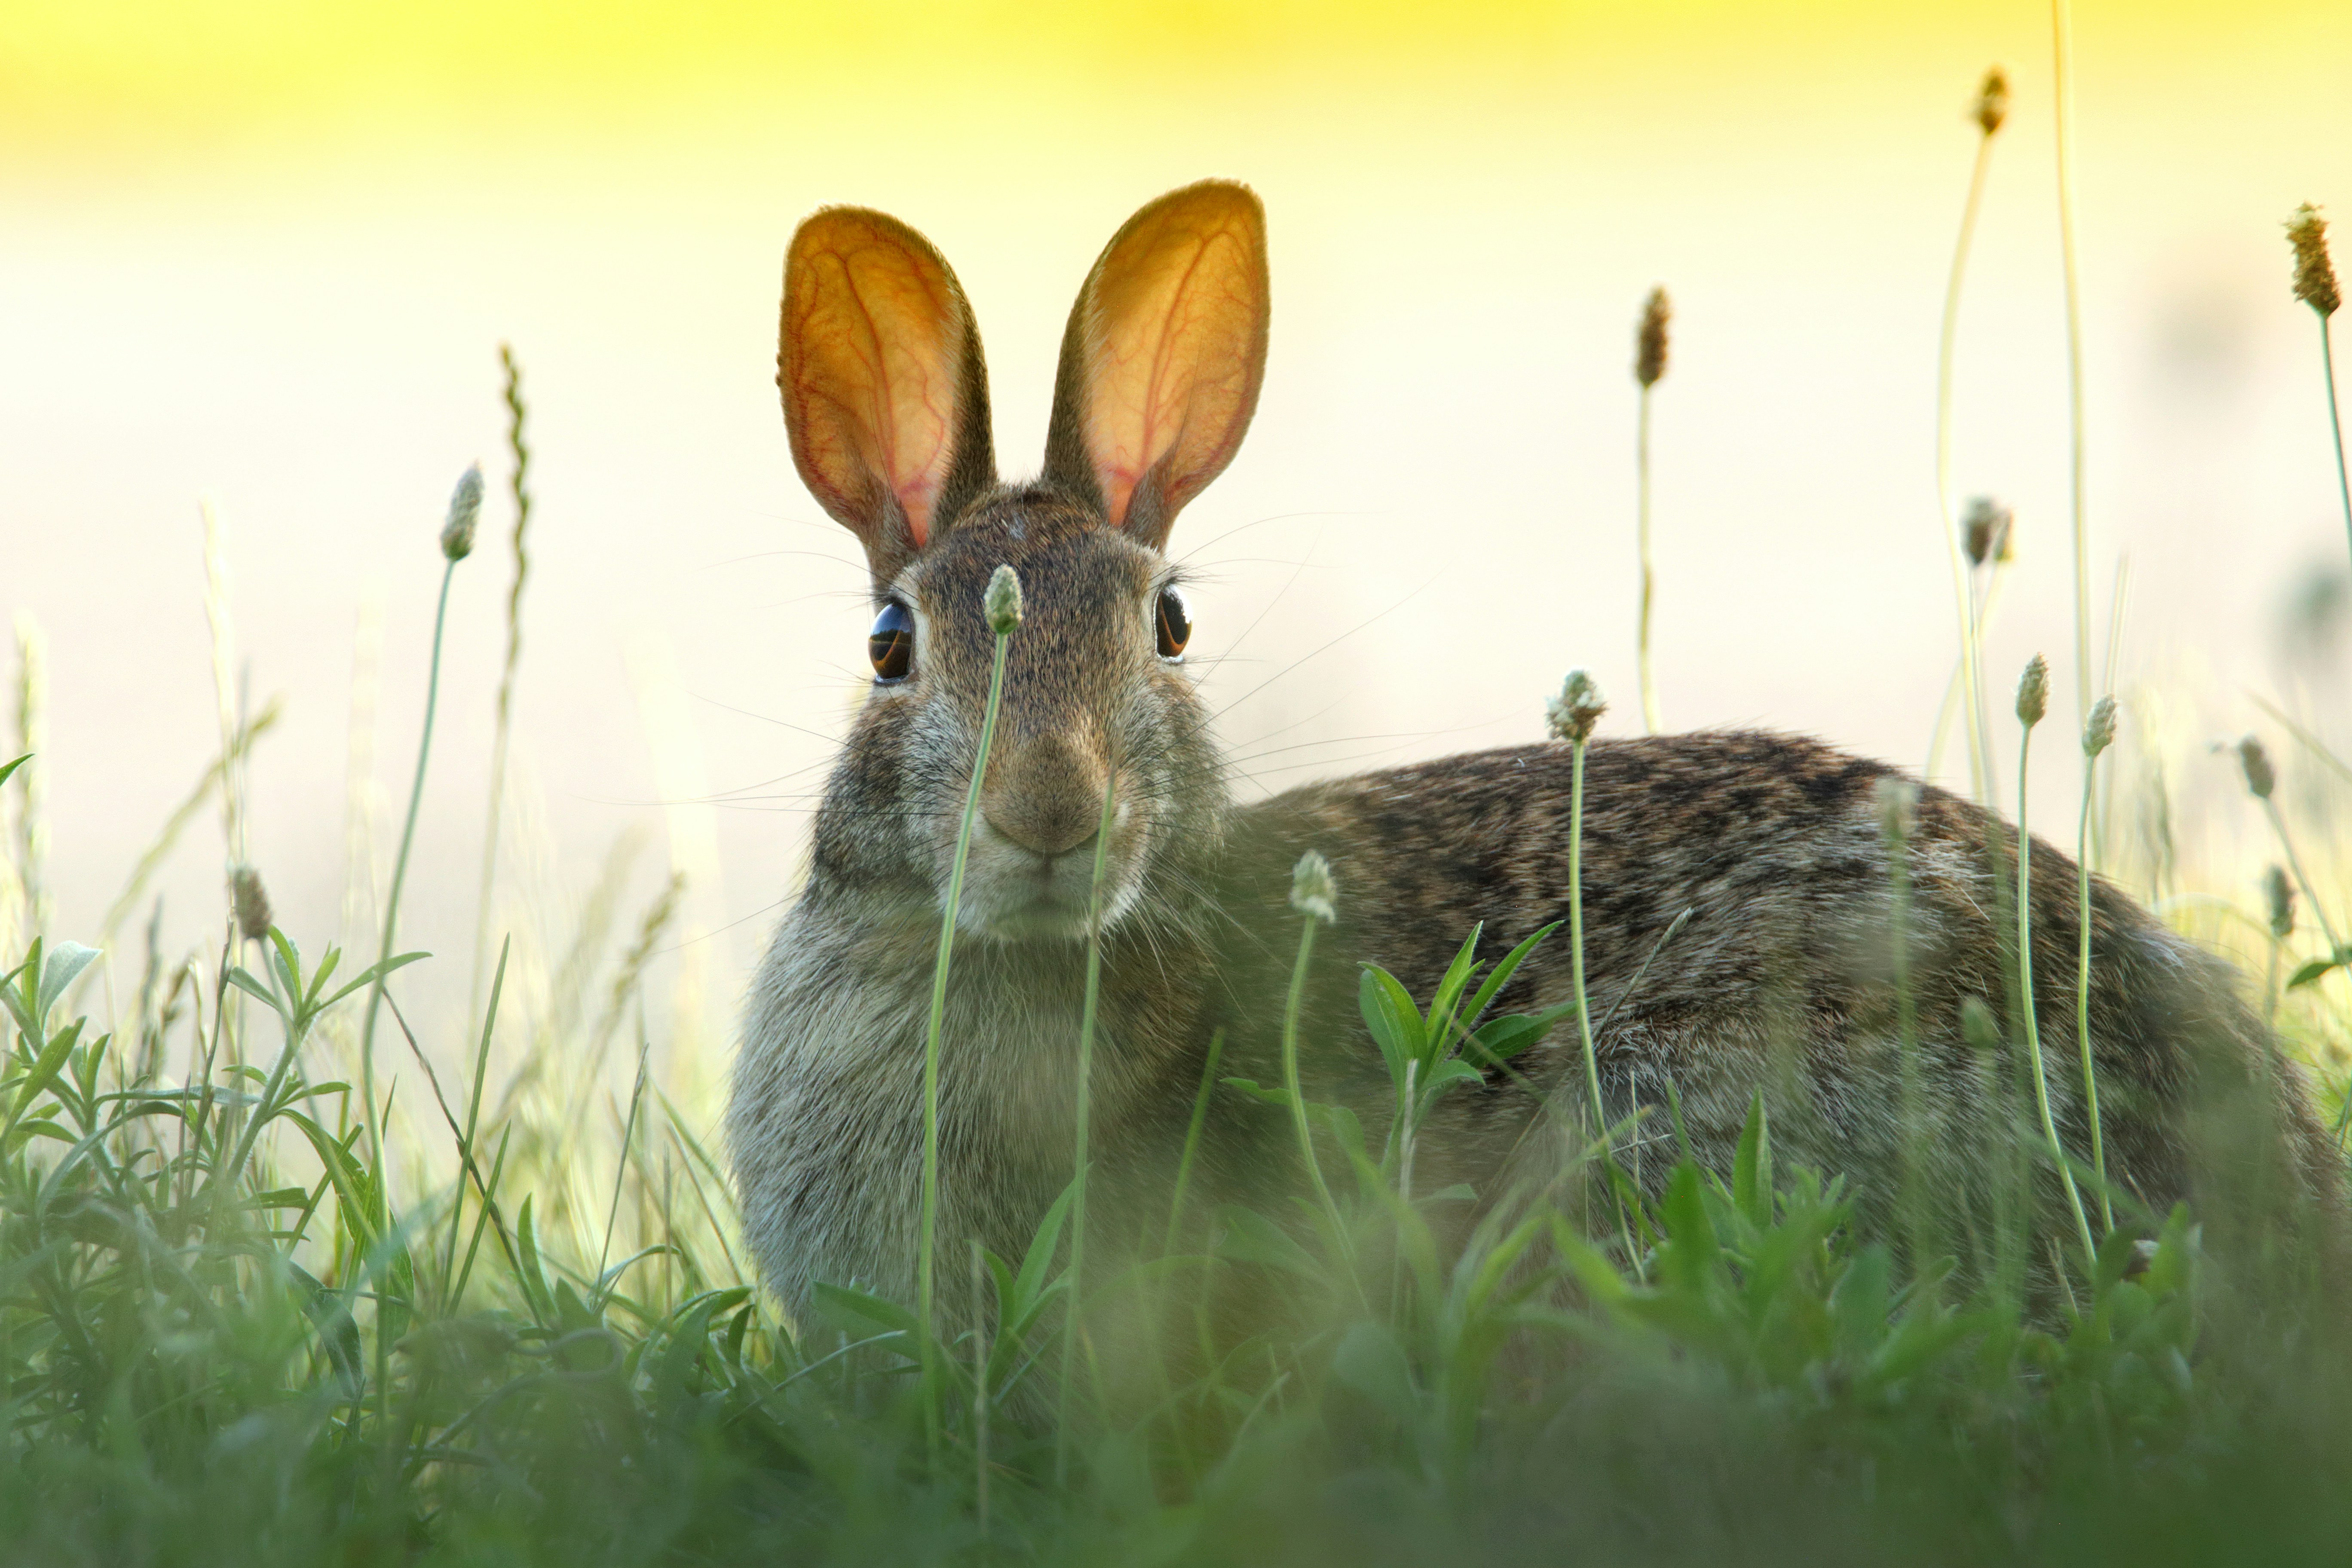
\includegraphics[width=\linewidth,padding=0cm 0cm 0cm 0cm]{bunny-3.jpg}\vfill}
        \end{column}
      \end{columns}
\end{frame}


\begin{frame}{ChronoTrigger: Changes in Rosenpass}
  \begin{columns}[fullwidth,c]

    \begin{column}{.2\linewidth}
      \rlap{\includegraphics[height=\extendedframetextheight,page=7,clip=true,trim=20 60 382 93]{rosenpass-wireguard-attack-types}}
    \end{column}

    \begin{column}{.2\linewidth}
      \rlap{\includegraphics[height=\extendedframetextheight,page=7,clip=true,trim=382 60 20 93]{rosenpass-wireguard-attack-types}}
    \end{column}

    \begin{column}{.56\linewidth}
    \small
      \begin{itemize}
        \item InitHello is unauthenticated because responder still needs to encapsulate secret with initiator key
        \item since InitHello is unauthenticated, retransmission protection is impossible
        \item responder state is moved into a cookie called \emph{Biscuit}; this renders the responder stateless
        \item retransmission of InitHello is now easily possible, but does not lead to a state disruption attack
        \item[$\Rightarrow$] stateless responder prevents ChronoTrigger attack
      \end{itemize}
    \end{column}
  \end{columns}
\end{frame}

\begin{frame}{Rosenpass Key Derivation Chain: Spot the Biscuit}
  \centering
  \includegraphics[height=\extendedframetextheight]{rosenpass-whitepaper-hashing-tree}
\end{frame}


\begin{frame}{Rosenpass Protocol Messages: Spot the Biscuit}
\centering
    \includegraphics[height=\extendedframetextheight]{rosenpass-whitepaper-message-types}
\end{frame}

  % \begin{itemize}
  %   \item Attacker trying to perform a protocol-level DoS attack
  %   \item Attacker may observe messages
  %   \item Attacker may insert messages, but they may not drop or modify messages
  %   \item Halfway between an active and passive attacker:
  %   \begin{itemize}
  %   \item For a fully active attacker state disruption is trivial; they can just drop messages
  %   \end{itemize}
  % \end{itemize}
